\documentclass[conference]{IEEEtran}
\usepackage{graphicx} % Required for inserting images
\usepackage[numbers]{natbib}
\usepackage[brazil]{babel}
\usepackage[utf8]{inputenc}    % Suporte a acentos (para versões antigas do LaTeX)
\usepackage[T1]{fontenc}       % Saída correta de acentos e cedilha
\usepackage{tabularx}
\usepackage[a4paper, left=2.5cm, right=2.5cm, top=3cm, bottom=3cm]{geometry}
\usepackage{hyperref}




\title{OffScan: Desenvolvimento de uma Ferramenta para Testes Ofensivos de Redes em Rust e C}
\author{\IEEEauthorblockN{Oliver Ribeiro Calazans Jeronimo}
\IEEEauthorblockA{Natal, Brazil \\
oliver.calazans@academico.ifrn.edu.br}
\and
\IEEEauthorblockN{Rezembrim de Paula Soares}
\IEEEauthorblockA{Natal, Brazil \\
rezembrim.soares@ifrn.edu.br}
}
\date{December 2025}

\begin{document}
\maketitle



\begin{abstract}
Este artigo apresenta o OffScan, uma ferramenta unificada para testes ofensivos de redes implementada principalmente em Rust, com módulos complementares em C. Desenvolvida com foco em modularidade, desempenho e autonomia, a ferramenta reduz dependências externas através do uso direto de chamadas de sistema e implementação manual de construtores de protocolos. O OffScan integra funcionalidades essenciais como mapeamento de redes, escaneamento de portas, ataques de flooding (TCP, ICMP) e técnicas específicas para redes Wi-Fi (desautenticação, inundação de beacons). Os resultados em ambiente controlado demonstram sua eficácia, com taxas de envio superiores a 400.000 pacotes por segundo em redes cabeadas e sucesso na execução dos ataques sem fio. A ferramenta representa uma contribuição prática ao ecossistema de segurança ofensiva, oferecendo uma base sólida para desenvolvimentos futuros.
\end{abstract}




\section{Introdução}
Com o crescimento exponencial da conectividade e da complexidade das infraestruturas de rede, a segurança cibernética tornou-se uma preocupação crítica para organizações e indivíduos. Os ataques evoluíram em sofisticação, alguns já bem documentados e reportados, como os citados no trabalho de \citet{lari-anto} exigindo ferramentas eficazes de teste de penetração e análise de vulnerabilidades que permitam avaliar proativamente a resiliência dos sistemas.

Neste contexto, este projeto apresenta o desenvolvimento da ferramenta \textit{OffScan}, uma solução ofensiva para redes escrita em Rust, em sua maior parte, e C. A escolha da linguagem Rust justifica-se por sua segurança de memória, desempenho similar ao de linguagens como C e por seu fácil acesso ao sistema. Algumas partes foram desenvolvidas em C pois apresentam um desenvolvimento mais simples e fácil do que em Rust.

O \textit{OffScan} foi desenvolvido com foco em modularidade, desempenho e autonomia, reduzindo ao máximo as dependências externas por meio do uso direto de chamadas de sistema e da implementação manual de construtores e parsers de protocolos de rede. A ferramenta incorpora funcionalidades para testes ofensivos, incluindo varredura de portas, mapeamento de redes, captura e injeção de pacotes, ataques de flood em múltiplas camadas e técnicas específicas para redes sem fio, como desautenticação e mapeamento de pontos de acesso.

Este relatório documenta o processo de desenvolvimento do \textit{OffScan}, detalhando a evolução da arquitetura, as funcionalidades implementadas e os resultados obtidos em ambiente controlado. Além disso, discute as lições aprendidas, as limitações identificadas e as direções futuras para o projeto.

\section{Fundamentação teórica}

A segurança ofensiva de redes compreende um conjunto de técnicas e metodologias destinadas a identificar, explorar e relatar vulnerabilidades em sistemas e infraestruturas de rede, com o propósito proativo de fortalecer suas defesas. Diferente da segurança defensiva, que visa proteger sistemas contra ataques, a abordagem ofensiva simula as ações de adversários reais para avaliar a resiliência dos mecanismos de proteção. Como mostrado no trabalho de \citet{offsec-emulation}, a área da segurança vem ganhando atenção por se mostrar eficiente e ajudar no treinamento de equipes e refinamento nas técnicas de detecção de ataques.

Neste projeto, a segurança ofensiva é aplicada por meio de ferramentas que realizam varreduras, explorações e testes de estresse em protocolos de rede, tanto em ambientes cabeados quanto sem fio. Técnicas como flooding (inundação), deautenticação em redes 802.11, spoofing (falsificação) de endereços IP e MAC são fundamentais para o teste de penetração, explorando falhas em protocolos, configurações inadequadas ou limitações de implementação.

Para a implementação de uma ferramenta ofensiva eficaz, é essencial o domínio dos protocolos de rede que atuam em diversas camadas do modelo TCP/IP. O TCP (\textit{Transmission Control Protocol}), protocolo orientado a conexão da camada de transporte, é alvo de técnicas como varredura e flooding. O UDP (\textit{User Datagram Protocol}), não orientado a conexão, permite varredura de portas com payloads específicos, explorando sua natureza \textit{connectionless}. O ICMP (\textit{Internet Control Message Protocol}), utilizado para diagnóstico, serve de base para ataques de flooding e técnicas de reflexão. Para redes sem fio, o padrão IEEE 802.11 (Wi-Fi) é essencial, sendo explorado por meio da captura de beacons e ataques de desautenticação, que manipulam quadros de gerenciamento.

O ecossistema de segurança ofensiva conta com diversas ferramentas consolidadas, cada uma com seus pontos fortes e limitações. Ferramentas como Nmap, para varredura de rede, e Scapy, para manipulação de pacotes em Python, são amplamente utilizadas, mas podem apresentar limitações de desempenho ou modularidade. Suítes como Aircrack-ng focam em redes Wi-Fi, mas com integração limitada a ambientes cabeados. Observa-se uma lacuna para uma ferramenta unificada.

A linguagem de programação Rust surge como uma escolha estratégica para o desenvolvimento de ferramentas de segurança ofensiva devido a um conjunto singular de vantagens. Seu sistema de propriedade (\textit{ownership}) e empréstimo (\textit{borrowing}) garante segurança de memória em tempo de compilação, prevenindo vulnerabilidades comuns como \textit{buffer overflows} e \textit{use-after-free}, problemas frequentes em linguagens como C/C++. Rust gera código máquina otimizado com desempenho similar a essas linguagens de baixo nível, crucial para operações de alta velocidade como flooding e varredura massiva. A linguagem também oferece concorrência segura, prevenindo data races em tempo de compilação, o que permite a implementação robusta de técnicas \textit{multithreading}. A interoperabilidade eficiente com C via FFI (\textit{Foreign Function Interface}) permite acesso direto a sockets brutos e chamadas de sistema. A combinação de desempenho, segurança e um ecossistema de desenvolvimento produtivo faz de Rust uma base ideal para construir ferramentas ofensivas confiáveis e eficientes.
\section{Metodologia}
Esta seção descreve a metodologia adotada para o desenvolvimento da ferramenta \textit{OffScan}, detalhando o ambiente de desenvolvimento, a arquitetura do sistema, as funcionalidades implementadas, os procedimentos de teste e os métodos de coleta de dados.

\subsection{Ambiente de Desenvolvimento}
O desenvolvimento do \textit{OffScan} foi realizado em um ambiente Linux (Debian 12 e 13), sistema operacional escolhido devido à sua compatibilidade com sockets brutos e chamadas de sistema de baixo nível necessárias para operações de rede ofensivas. As linguagens de programação utilizadas foram Rust (versão estável 1.89.0), selecionada por suas garantias de segurança de memória e desempenho, e C, devido à maturidade de suas bibliotecas de integração com o subsistema \textit{Netlink} e ao acesso direto aos cabeçalhos nativos do kernel, o que facilita a configuração de interfaces de rede sem fio.

As principais ferramentas e bibliotecas/crates utilizadas incluem:
\begin{itemize}
    \item \textbf{Cargo} Sistema de build e gerenciador de pacotes do ecossistema Rust. Versão 1.89.0.

    \item \textbf{pcap}: Crate para criação de sniffers de pacotes de rede. Versão 2.3.0.

    \item \textbf{libc}: Crate para chamadas diretas ao sistema, substituindo abstrações de alto nível. Versão 0.2.177.

    \item \textbf{clap}: Framework para parsing de argumentos de linha de comando. Versão 4.5.

    \item \textbf{rand}: Crate para geração de valores aleatórios. Usada para a criação de IPs, MACs e outros valores aleatórios. Versão 0.8.5.

    \item \textbf{libpcap-dev}: Biblioteca a nível de sistema usada para captura de pacotes. Usada pela crate \texttt{pcap}

    \item \textbf{libnl-3-dev \& libnl-genl-3-dev}: Bibliotecas a nível de sistema usadas para se comunicar com o kernel via netlink para configuração rede.
\end{itemize}


\subsection{Arquitetura da ferramenta}
A arquitetura do \textit{OffScan} segue um design modular, organizado em componentes especializados que colaboram para executar operações ofensivas complexas. Seus principais módulos consistem em:

\begin{itemize}
    \item \textbf{Motores}: São blocos onde são executadas operações usando as informações e funções dos outros módulos de forma coordenada com as próprias para executar um scanner ou ataque.
    
    \item \textbf{Construtores de pacotes/quadros 802.11}: Responsáveis pela construção manual de pacotes de rede em todas as camadas (Ethernet, IP, TCP/UDP/ICMP) e dos quadros 802.11.

    \item \textbf{Sockets Brutos}: Responsáveis por enviar os pacotes brutos.

    \item \textbf{Sniffer}: Responsável por capturar pacotes ou quadros diretamente de uma interface.

    \item \textbf{Dissecadores}: Responsáveis por extrair informações dos pacotes/beacons.

    \item \textbf{Generadores}: Blocos de código responsávies por gerar valores aletórios como IPs, MACs e portas.

    \item \textbf{Provedor de informações}: Responsávies por fornecer informações interfaces de rede.

    \item \textbf{Controlador de interface}: Responsável por alterar as configurações das interfaces.

    \item \textbf{Módulos em C}: Apesar de maior parte do projeto ser escrita com a linguagem Rust, algumas funções foram feitos usando a linguagem C por ter um desenvolvimento mais fácil e por melhor integração com chamas a parte do sistema resposável pela configuração da interface de rede sem fio (netlink/nl80211).

    \item \textbf{Utilitários}: São funções isoladas e pequenas que são usadas em várias partes do código. Porém, são pequenas e específicas. Não se encaixando nas outras categorias.
\end{itemize}


\subsection{Fluxo de execução}
A ferramenta opera como uma aplicação de linha de comando, onde cada funcionalidade é acessada via subcomandos específicos. O fluxo geral inclui: (1) parsing de argumentos, (2) inicialização dos módulos necessários, (3) execução da operação principal (varredura, ataque ou análise), e (4) apresentação estruturada dos resultados.
\section{Funcionalidades}
A ferramenta tem seu foco em ataques a redes e a infraestrutura. Mas, também conta com alguns scanners que são úteis para fornecer informações para serem usadas nos ataques. Elas são:


\subsection{Ataque de Desautenticação}
Um flooder de frames IEEE 802.11 de gerenciamento usado para desautenticar dispositivos da rede. Esse ataque explora uma vulnerabilidade fundamental no protocolo 802.11, que gerencia as comunicações Wi-Fi. Ele é possível devido a duas características principais do protocolo:

\begin{itemize}
    \item Os quadros de gerenciamento, como os de autenticação e desautenticação, são enviados sem criptografia, mesmo em redes protegidas por WPA2 ou WPA3.

    \item O padrão Wi-Fi original não exige que os dispositivos verifiquem se um quadro de desautenticação foi enviado pelo ponto de acesso legítimo.
\end{itemize}

Um atacante pode enviar quadros de desautenticação forjados para um dispositivo (cliente) e/ou para o ponto de acesso (AP), fingindo ser a outra parte legítima da conexão. O dispositivo ou o AP aceita esses quadros falsificados como se fossem legítimos, pois não há um mecanismo de verificação de origem. Essa falha é usada em combinação com outros ataques como o ataque \texttt{kr00k} \cite{kr00k}, \texttt{KRACK} \cite{krack} e \texttt{evil-twin} \cite{evil-twin}.

O \textit{OffScan} usa dessas falhas para executar o ataque. Ele cria os frames de desautenticação usando as informações passadas pela linha de comando e envia os frames em um loop infinito para o host alvo, se passando pelo AP, e para o AP, se passando pelo host alvo.




\subsection{Inundador de Beacons}
Beacons são quadros (frames) enviados por roteadores de redes Wi-Fi para se apresentarem e enviarem informações necessárias para que dispositivos possam se conectar as suas redes sem fio.

O inundador de beacons cria vários desses beacons com informações falsas para que os dispositivos ao alcance recebem esses beacons e os processem como se fossem redes reais. Isso faz com que a lista de redes disponíveis fique maior e confunda os usuários, o que se enquadra em um ataque de confusão de SSID \cite{confusion-attack}. Uma das informações que o inundador usa é nome de rede (BSSID) que pode ser de uma rede real ou não. Para evitar filtragem de redes pela repetição do mesmo BSSID, o código cria variações do nome passado, alterando algumas letras de maiúscula para minúscula, e o inverso também. Assim como o ataque de desautenticação, esse flooder é comumente usado em conjunto com outras técnicas.




\subsection{Inundador de pacotes Ping}
Esse flooder usa do protocolo ICMP, mais especificamente as mensagens Echo/Request para um ou mais alvos. 

O ICMP é um protocolo fundamental de camada de rede usado para diagnósticos (como o comando ping) e mensagens de erro. Ele é projetado para ser simples e leve, sem mecanismos de autenticação ou limites de taxa integrados. Para cada solicitação de eco (ping) recebida, o dispositivo de destino deve enviar uma resposta de eco, consumindo recursos. Além da natureza do protocolo, o spoofing de IP contribui para esse ataque, pois dificilmente uma rede implementa mecanismos que previnem spoofing de IP. 

O \textit{OffScan} cria os pacotes com IPs spoofados e os envia na rede. Ele pode enviar esse pacotes para um único host, se passando por dispositivos aleatórios, ou para IPs aleatórios.

Podem haver limitadores como largura de manda e controle dos meios de comunicação. Devido a possibilidade de falsificação de IP, é possível usar a técnica de ataque "\texttt{smurf}" \cite{smurf}. Essa técnica de amplificação de ataque é feita colocando o endereço do alvo nos campos de endere de origem e nos endereços de destino é colocado em broadcast. Assim, todos os dispositivos da rede enviam pacotes Echo Reply para o alvo \cite{tecnica-smurf}. A amplificação do ataque depende da quantidade de dispositivos na rede. Por exemplo, m uma rede /24, com todos os IPs ativos, a aplificação tem efeito de 252 vezes.

Também é possível executar ataques de reflexão, já que é possível \textit{spoofar} ambos os IPs dos pacotes. Os pacotes são enviados à um terceiro dispositivo e ele envia as respostas para o alvo.



\subsection{Inundador de pacotes TCP (SYN)}
Esse tipo de flooder é muito usado em ataques DDoS. O exemplo mais famoso do uso dessa técnica é pelo Botnet Mirai \cite{botnet-mirai}. A vulnerabilidade de SYN flooding foi formalmente documentada e analisada, com código de exploração divulgado na Phrack Magazine em 1996 (RFC 4987) \cite{tecnica-tcp-syn}. Um flooder de pacotes TCP SYN direcionado a um host para um porta especificada.

Os ataques de TCP flood são possíveis devido a
vulnerabilidades inerentes ao processo de estabelecimento de conexão do protocolo TCP, especificamente o \textit{three-way handshake} (aperto de mão em três vias).

Para cada solicitação SYN recebida, o servidor/alvo reserva uma quantidade limitada de recursos em sua fila de espera (backlog). Um grande volume de solicitações incompletas esgota rapidamente esses recursos, impedindo que o servidor aceite novas conexões legítimas, o que resulta em negação de serviço.

Em redes domesticas, o flooder é capaz de reduzir o throughput e, alguns casos, de paralisar a rede por sobrecarregar o AP. Em redes corporativas os desafios são maiores já que a rede é mais controlada, monitorada e robusta.


\subsection{Mapeador de rede}
Apesa de não ser um ataque, e sim uma técnica de reconhecimento \cite{ip-scanning}, ele é extremamente útil para serem usadados em ataque e/ou tomadas de decisão. Um mapeador de redes usa uma técnica de enviar pacotes especificos e analisar as respostas recebidas. No caso de uma escaneamento ativo.

O mapeador de rede do \textit{OffScan} envia pacotes ICMP, TCP e UDP (por padrão, é possível escolher quais dentre os três será(ão) usado(os)) para todos os IPs da rede, ou de um range especificado. O gerador recebe o CIDR (baseado na interface que será usada) ou um range específico e calcula todos os IPs possíveis e entrega um iterador para ser usado nos probes.

Durante o envio dos pacotes, um sniffer fica capturando as respostas em uma thread separada. Ele possui um filtro BPF (\textit{Berkley Packet Filter}) que busca por pacotes IPv4 e que contenham endereços de IP dentro do range especificado por um CIDR. Esse CIDR é criado basedo no primeiro e último IPs gerados pelo módulo \texttt{Ipv4Iter}. Assim, deixando a captura por pacotes mais especifica.


\subsection{scanner de portas}
Uma técnica muito usada para descobrir portas abertas e depois descobrir qual serviço está sendo executado naquela porta para poder explora-lo \cite{port-scan}.

Esse comando envia pacotes TCP ou UDP para um range de portas, especificados ou pré definidos, para descobrir quais estão abertas.

O \textit{OffScan}, no scanner de portas TCP, usa a técnica \textit{stealth}. Ela consistem em enviar pacotes SYN, o primeiro pacotes do \textit{three-way-handshake}. Enquanto os pacotes estão sendo enviados, um sniffer fica capturando apenas os respostas SYN-ACK, que é o segundo pacotes do \textit{handshake}. Logo após o envio, as respostas são dissecadas para decobrir quais portas responderam como abertas.

No scanner de de portas UDP, o processo é diferente. Pela natureza \textit{stateless} do protocolo e seu objetivo de rapidez e simplicidade, são necessários payloads específicos para receber a confirmação das portas abertas. O protocolo UDP tem respostas diferentes do TCP. Quando uma porta está fechada, normalmente, um pacote ICMP é enviado com a \textit{flag Port Unreachable} (porta inalcançável). Quando a porta está aberta, o protocolo não responde a pacotes em payloads. Por essa razão é necessário o uso de payloads especificos para os serviços que estão sendo oferecidos nas portas, com algumas ressalvas. Se o payload não for compatível com o serviço da porta, pode não haver resposta. Os payloads usados no scanner UDP do \textit{OffScan} são baseados em serviços que rodam em portas padronizadas.


\subsection{Mapeador de redes Wi-Fi}
O reconhecimento das redes Wi-Fi está cada vez mais sendo usado por atacantes por ser um vetor/porta inicial de ataque \cite{wifi-vec}. Buscar informações sobre as redes disponíveis pode revelar informações de má configuração e/ou pontos fracos da infraestrutura \cite{sec-info}.

O mapedor de redes Wi-Fi tem como objetivo mostrar o BSSID e o canal de cada rede wifi ao alcance. Essas informações são úteis para o ataque de desautenticação. 

O mapeador tem dois submódulos, um que busca as informações do sistema (\texttt{SysSniff}) e outro que captura os beacons com o sniffer (\texttt{MonitorSniff}).

O \texttt{SysSniff} usa um módulo feito em C, que se comunica com o kernel a partir do netlink, para ativar o trigger responsável por fazer a interface escanar todos os canais pegando os beacons das redes. Após isso, o módulo busca as informações das redes diretamente o kernel e os entrega para o submódulo em Rust. Então, as funções do submódulo apenas formatam as informações recolhidas do sistema e depois as mostra.

Já o \texttt{MonitorSniff} faz o mesmo processo do sistema, porém, faz todo o trabalho manualmente e com a interface no modo monitor. Ele inicia o sniffer na interface e entra em um loop que fica alterando o canal da interface periodicamente. Após escanar cada interface, o sniffer é fechado e os pacotes são processados e as informações são formatadas e apresentadas.

Os dois submódulos apresentam os mesmos resultados, porém, o \texttt{SysSniff} só pode ser usado quando a interface está no modo managed (modo no qual está conectada à uma rede), dispensando a necessidade de colocar a interface no modo monitor. Já o \texttt{MonitorSniff} só funciona com o modo monitor.


\subsection{Informações de Rede e Interface}
Essa funcionalidade tem como objetivo mostrar algumas informações da interface e da rede, se estiver conectada, sem a necessidade de escanar a rede. As informações que são apresentadas são:

\begin{itemize}
    \item Nome da interface
    \item Estado da interface (UP, DOWN, ETC)
    \item Tipo (Ethernet, Wireless, etc)
    \item Endereço MAC
    \item Endereço de IP
    \item Endereço da rede e mascara (CIDR)
    \item Quantidade de IPs válidos
    \item MTU (Unidade Máxima de Transmissão)
    \item Endereço MAC do gateway
    \item Endereço de IP do gateway
\end{itemize}

Essas informações são buscadas de origens diferentes. Nome, estado, tipo, MAC e MTU são copiadas dos arquivos \texttt{/sys/class/net/<interface>}. Já os endereços de IP e MAC do gateway são copiados de arquivos que ficam nos diretórios \texttt{/proc/net/}. Já o IP e o endereço da rede com a máscara são conseguidos atravez de chamadas ao sistema usando a crate \texttt{libc}. E a quantidade de IPs válidos é calculada através do CIDR.

Essas informações são úteis para serem usadas pelos outros comandos e/ou para tomada de decisão.
\section{Resultados}
Os resultados da execução de cada função mostra como o está o funcionamento do sua funcionalidades. 

\subsection{Amostra das execuções}

\subsubsection{Ping Flooder}
O flooder de pacotes Ping mostrou um bom funcionamento. No exemplo abaixo mostra uma rápida execução desse flooder onde os endereços de IP e MAC do alvo foram informados e o endereço MAC de origem usado foi o local, MAC da interface usada.
\begin{figure}[h]
    \centering
    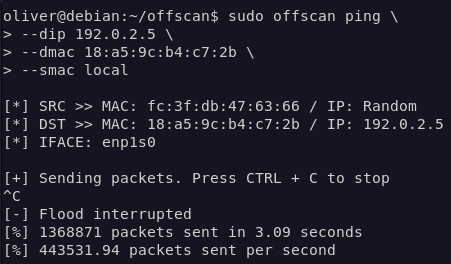
\includegraphics[width=0.45\textwidth]{fotos/ping.png}
    \caption{Execução do flooder de pacotes Ping}
\end{figure}


\subsubsection{TCP Flooder}
O flooder de pacotes TCP SYN também mostrou bom funcionamento. No exemplo abaixo mostra uma rápida execução desse flooder onde, além das informações usadas no exemplo anterior, a porta foi informada.
\begin{figure}[h]
    \centering
    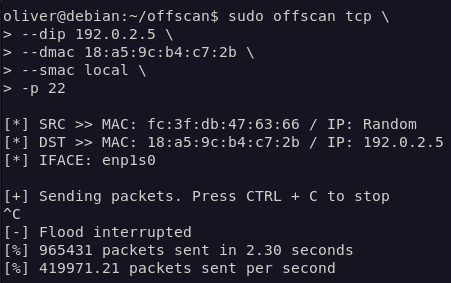
\includegraphics[width=0.45\textwidth]{fotos/tcp.png}
    \caption{Execução do flooder de pacotes TCP}
\end{figure}


\subsubsection{Ataque de desautenticação}
O ataque demonstrou ser eficaz em provocar a desassociação do cliente do ponto de acesso. O tempo de reação do dispositivo alvo fica entre 15 e 30 segundos.
\begin{figure}[h]
    \centering
    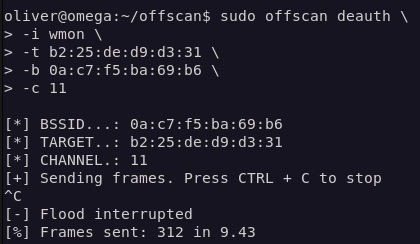
\includegraphics[width=0.45\textwidth]{fotos/deauth.png}
    \caption{Execução do mapeador de rede}
\end{figure}



\subsubsection{Mapeador de redes}
No exemplo abaixo, apenas o comando para mapear a rede foi informado. Com isso, a interface padrão é usada e a partir do IP e da mascara da rede, todos os IPs da rede são calculados para serem escaneados.
\begin{figure}[h]
    \centering
    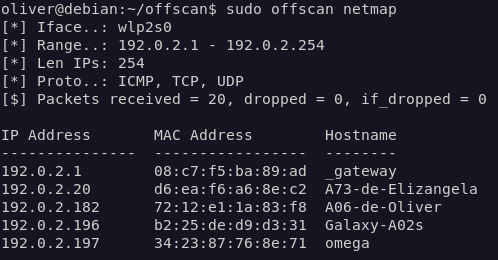
\includegraphics[width=0.46\textwidth]{fotos/netmap.png}
    \caption{Execução do mapeador de rede}
\end{figure}


\subsubsection{Informações de Rede e Interface}
No exemplo abaixo o comando \texttt{info} foi executado. Ele mostra informações da interface que foi escolhida e da rede ao qual está conectada, se estiver.
\begin{figure}[h]
    \centering
    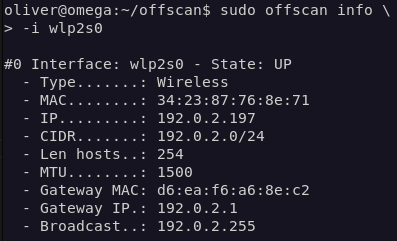
\includegraphics[width=0.46\textwidth]{fotos/info.png}
    \caption{Execução do comando \texttt{info}}
\end{figure}


\subsubsection{scanner de portas}
Na amostra abaixo, o scanner varreu as portas do gateway. Veja que ele apenas mostra qual a porta aberta, não o serviço.
\begin{figure}[h]
    \centering
    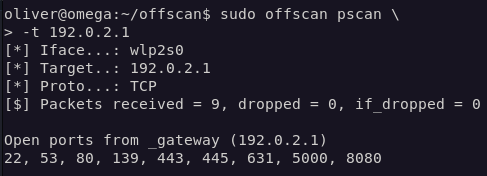
\includegraphics[width=0.46\textwidth]{fotos/pscan.png}
    \caption{Execução do scanner de portas}
\end{figure}


\subsubsection{Mapeador de redes Wi-Fi}
No exemplo desse comando foram alterados o nome da rede (SSID) e parte do BSSID de cada rede para preservar a privacidade. A imagem abaixo mostra como o comando mostra as informações que pegou de cada rede Wi-Fi.
\begin{figure}[h]
    \centering
    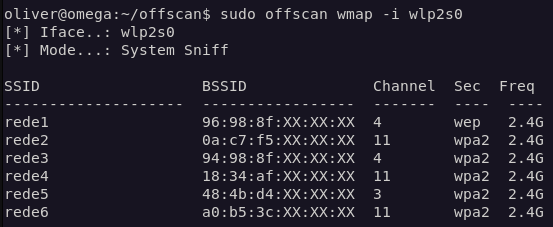
\includegraphics[width=0.46\textwidth]{fotos/wmap.png}
    \caption{Execução do mapeador de redes Wi-Fi}
\end{figure}


\subsubsection{Flooder de beacons}
O flooder de beacons se mostrou muito eficiente como mostra a imagem abaixo. Nela, é possível ver algumas das muitas redes inexistentes que os beacons transmitiram.
\begin{figure}[h]
    \centering
    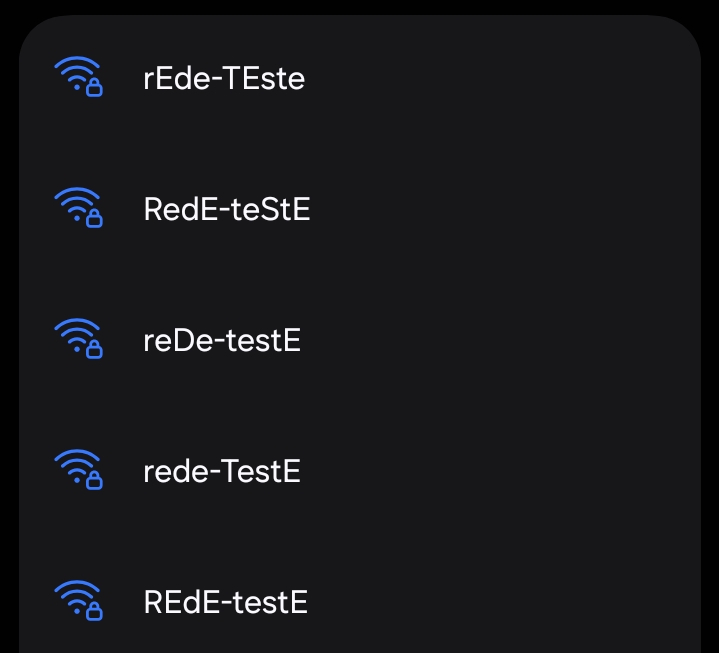
\includegraphics[width=0.46\textwidth]{fotos/beacon.jpg}
    \caption{Execução do flooder de beacons}
\end{figure}


\subsection{Análise dos resultados}
Com base nas execuções, observou-se que: 

\begin{itemize}
    \item \textbf{Flooder TCP e ICMP}: Ambas as funcionalidades alcançaram taxas médias de envio superior a 400.000 pacotes por segundo em redes cabeadas.
    
    \item \textbf{Flooder de beacons}: A taxa de envio foi limitada intencionalmente para evitar a saturação do espectro e permitir a visualização clara das redes falsas. Apesar dessa limitação, a funcionalidade mostrou-se eficaz, com múltiplos dispositivos detectando as redes falsas criadas.
    
    \item \textbf{Ataque de desautenticação}: O tempo médio para desconexão dos dispositivos-alvo variou entre 15 e 30 segundos. Notou-se que, em alguns casos, foi necessário reiniciar o envio dos quadros para manter a desconexão, indicando uma possível reassociação automática do cliente.

    \item \textbf{Mapeamento Wi-Fi}: A ferramenta obteve sucesso em detectar todas as redes sem fio dentro do alcance do dispositivo, tanto no modo \texttt{SysSniff} (através da API do kernel) quanto no modo \texttt{MonitorSniff} (interface em modo monitor).
    
    \item \textbf{Mapeador de redes}: Demonstrou alta eficácia na descoberta de hosts ativos, identificando corretamente dispositivos conectados na rede através de múltiplos protocolos (ICMP, TCP, UDP).
    
    \item \textbf{scanner de portas}: Mostrou-se eficiente na identificação de portas abertas, tanto com a técnica SYN (TCP) quanto com payloads específicos (UDP). A taxa de falsos positivos foi baixa, e o desempenho foi satisfatório para varreduras em intervalos de portas comuns.
\end{itemize}
\section{Melhorias e Trabalhos Futuros}

Com base no desenvolvimento e nos testes realizados com o OffScan, foram identificadas várias oportunidades de melhoria e direções para trabalhos futuros:

\subsection{Otimização de Desempenho}

Durante a análise de desempenho com a ferramenta \texttt{perf}, observou-se que aproximadamente 99\% do tempo de execução é gasto no contexto do kernel, devido às frequentes chamadas de sistema. Cada chamada exige uma mudança de contexto entre espaço do usuário e kernel, o que consome recursos computacionais e limita a taxa de envio de pacotes.

Para mitigar esse problema, planeja-se:

\begin{itemize}
    \item \textbf{Batch de operações}: Agrupar múltiplas operações de envio ou recepção em uma única chamada de sistema, reduzindo o número total de mudanças de contexto.
    
    \item \textbf{Sockets de alta performance}: Utilizar sockets do tipo \texttt{PF\_PACKET} com configurações otimizadas, como buffers circulares (ring buffers) para reduzir a sobrecarga.
    
    \item \textbf{Acesso direto ao hardware}: Explorar o uso de DPDK (Data Plane Development Kit) ou XDP (eXpress Data Path) para processamento de pacotes em alta velocidade, contornando completamente a pilha de rede do kernel.
\end{itemize}

\subsection{Expansão de Funcionalidades}

Atualmente, o OffScan foca em um conjunto básico de ataques. Para torná-lo mais versátil, planeja-se adicionar:

\begin{itemize}
    \item \textbf{Ataques de camada de aplicação}: Implementar ataques específicos para protocolos como HTTP, DNS, SIP e VoIP, incluindo técnicas de injeção e amplificação.
    \item \textbf{Técnicas de evasão}: Adicionar funcionalidades para contornar sistemas de detecção de intrusão (IDS/IPS) e firewalls, como fragmentação de pacotes, criptografia de tráfego e uso de proxies.
    \item \textbf{Suporte a IPv6}: Estender todas as funcionalidades para suportar o protocolo IPv6, incluindo varredura, flooding e mapeamento de redes.
    \item \textbf{Ataques a redes mesh e ad-hoc}: Desenvolver técnicas específicas para redes mesh 802.11s e redes ad-hoc, que possuem características diferentes das redes infraestrutura tradicionais.
\end{itemize}

\subsection{Aprofundamento dos Ataques Existentes}

Os ataques atualmente implementados podem ser aprimorados para aumentar seu impacto e eficácia:

\begin{itemize}
    \item \textbf{Ataque de desautenticação}: Implementar variações do ataque, como deautenticação em massa para múltiplos clientes simultaneamente, e técnicas para manter a desconexão por períodos prolongados.
    \item \textbf{Flooders}: Adicionar opções para modificar a taxa de envio dinamicamente, baseado na resposta da rede, e suporte a múltiplos alvos simultaneamente.
    \item \textbf{Escaneamento de portas}: Incluir detecção de serviços e versões, além de suporte a técnicas de escaneamento mais discretas (\textit{stealth scanning}) e distribuição de varredura por múltiplos hosts.
\end{itemize}

\section{Conclusão}

O desenvolvimento do \textit{OffScan} demonstrou a viabilidade de criar uma ferramenta unificada para testes ofensivos de redes utilizando Rust como linguagem principal. A ferramenta implementou com sucesso funcionalidades essenciais como flooding de pacotes, mapeamento de redes, escaneamento de portas e ataques a redes Wi-Fi, alcançando desempenho satisfatório em ambiente controlado.

Os resultados confirmaram as vantagens da escolha de Rust, particularmente em termos de segurança de memória e desempenho, enquanto a integração com C permitiu acesso a APIs de baixo nível do kernel. Embora existam oportunidades de otimização e expansão, o \textit{OffScan} representa uma contribuição válida para o ecossistema de ferramentas de segurança ofensiva, oferecendo uma base sólida para desenvolvimentos futuros.

Trabalhos subsequentes poderão focar na redução do \textit{overhead} de chamadas ao sistema e na implementação de novos tipos de ataques, transformando a ferramenta em uma solução mais completa para profissionais de segurança.


\bibliographystyle{plainnat}
\bibliography{ref}
\end{document}